% Created 2014-08-26 Tue 11:59
\documentclass[colorlinks=true,urlcolor=blue,linkcolor=blue,citecolor=red]{article}
\usepackage[utf8]{inputenc}
\usepackage{lmodern}
\usepackage[T1]{fontenc}
\usepackage{fixltx2e}
\usepackage{graphicx}
\usepackage{longtable}
\usepackage{float}
\usepackage{wrapfig}
\usepackage{rotating}
\usepackage[normalem]{ulem}
\usepackage{amsmath}
\usepackage{textcomp}
\usepackage{marvosym}
\usepackage{wasysym}
\usepackage{amssymb}
\usepackage{amsmath}
\usepackage[version=3]{mhchem}
\usepackage[numbers,super,sort&compress]{natbib}
\usepackage{natmove}
\usepackage{url}
\usepackage{minted}
\usepackage{underscore}
\usepackage[linktocpage,pdfstartview=FitH,colorlinks,
linkcolor=blue,anchorcolor=blue,
citecolor=blue,filecolor=blue,menucolor=blue,urlcolor=blue]{hyperref}
\usepackage{attachfile}
\usepackage{minted}
\usepackage{lmodern}
\usepackage{makeidx}
\usepackage[margin=1in]{geometry}
\author{Zhongnan Xu}
\date{14-8-2014}
\title{Tutorial to using \textsc{Quantum ESPRESSO} with the espresso.py module}
\begin{document}

\maketitle
\tableofcontents

\section{Introduction}
\label{sec-1}
The purpose of tutorial is instruct one how to perform first principles, density functional theory (DFT) calculations efficiently with the \textsc{Quantum-ESPRESSO} program along with the python wrapper \texttt{espresso.py}. The purpose of this guide, as of now, is \emph{not} instructional for\ldots{}

\begin{enumerate}
\item Physics behind implementations of DFT
\item Setting up specific atoms objects for calculations
\item Calculating physical or thermodynamic properties from DFT
\end{enumerate}

Instead, we will go over some of the nuts and bolts of successfully running DFT calculations. These topics include

\begin{enumerate}
\item Writing code for submitting, checking, and reading PWSCF and DOS calculations
\item Some parameter optimization tests
\item Dealing with common errors
\end{enumerate}

Therefore, it assumed that user has had some experience with ASE, and the explanations of constructing the atoms object will not be given.

\section{Installation}
\label{sec-2}
The \texttt{espresso.py} module requires both \textsc{QUANTUM-Espresso} and the Atomic Simulation Environment (ASE) to be installed and working on the system. These are both free and can be found at \url{http://www.quantum-espresso.org/} and \url{https://wiki.fysik.dtu.dk/ase/}, respectively. All python modules required are the same as listed for ASE.

Once the \texttt{espresso.py} module has been downloaded, just add this line to your path.

\begin{minted}[frame=lines,fontsize=\scriptsize,linenos]{bash}
export PYTHONPATH=path/to/espresso/espresso:$PYTHONPATH
\end{minted}

Note, the espresso folder within the overall \texttt{espresso.py} module folder (also named espresso) is the path that must be added.

\section{Performing calculations}
\label{sec-3}
\subsection{PWSCF calculations}
\label{sec-3-1}
The most common calculation you will be performing are Plane Wave Self-Consistent Field (PWSCF) calculations. In these calculations, we specify the atomic coordinates, pseudopotentials, and parameters, and it calculates for us important thermodynamic quantities such as the total energy, force, and stresses. After a successful calculation, we can then extract the data. Both performing and reading the calculation can be done with the \texttt{espresso.py} module. All code for reproducing this data can be found in the tutorials/input/PWSCF folder

Note, performing this calculation does not give us human readable information on the electronic structure besides basic information on band occupancies. Obtaining useful electronic structure information for the construction of band structures and density of states (DOS) require followup calculations from programs within the \textsc{QUANTUM-Espresso} module and will be summarized in following sections. However, it all starts with the \texttt{pwscf} command.

\subsubsection{The simplest possible example: H in a box}
\label{sec-3-1-1}
One of the simplest systems to calculate (though not necessarily the fastest) is an atom in a box. Because of the large size of the box and sharp gradients in the electronic density due to it being an atomic state, electronic convergence can be surprisingly slow. However, this is by far the easiest system to imagine, so we start with this to show the basics of running commands.

The beginning of the script will always start the same
\begin{minted}[frame=lines,fontsize=\scriptsize,linenos]{python}
from espresso import * # First import the module
\end{minted}

This command imports all of the commands you will ever need to run \textsc{QUATNUM-Espresso} calculations. This will be imported pretty early on.

After this, we need to construct our atoms object. This is done below. The H atom is at the (0, 0, 0) coordinate, and the cell is a cuboid with edge lengths 8, 9, and 10 $\AA$ long. We need a cuboid to break symmetry, which is required for finding the ground states of gaseous atoms. The box needs to be large enough to minimize neighbor interactions.

\begin{minted}[frame=lines,fontsize=\scriptsize,linenos]{python}
from ase.atoms import Atoms, Atom # Import the atoms object from ASE

atoms = Atoms([Atom('H', (0, 0, 0))],
              cell = (8, 9, 10))
\end{minted}

Now we run the calculation.

\begin{minted}[frame=lines,fontsize=\scriptsize,linenos]{python}
with Espresso('examples/output/H',         # With respect to the directory this script
                                           # is in, this is the directory where the
                                           # calculation will be taking place. The module
                                           # will automatically make the folders necessary.
                                           # Just assure the folder doesn't exist, and if it
                                           # does, that it's empty

              atoms=atoms,                 # This is where we put in the atoms object

              ecutwfc=60.0, ecutrho=600.0, # These are the kinetic energy cutoff parameters
                                           # These values determine heavily the convergence
                                           # of your calculation and therefore the time and
                                           # accuracy of your calculation. You should perform
                                           # convergence tests before performing large amounts
                                           # of studies.

              kpts=(1, 1, 1),              # This is how many kpoints in the x, y, and z
                                           # direction of the unit cell. Similar to ecutwfc
                                           # and ecutrho, the more kpoints the more converged
                                           # and expensive. Testing is recommended.

              occupations='smearing',      # This is to determing the smearing at electrons
                                           # at the fermi level. Typically we do smearing.

              smearing='gauss',            # The type of smearing we want. Typically its gauss
                                           # for insulators and mp (methfessel-paxton) for
                                           # metals.

              degauss=0.01) as calc:       # The width of the smearing. Will dicuss this value
                                           # later.
    calc.calculate()
\end{minted}

Performing this calculation will return one of four things.

\begin{enumerate}
\item The exception \texttt{EspressoSubmitted} \\ \\
   This means your job was successfully submitted! Whether its correctly running or not is a different story, and examples of this will be covered in later sections. If you submit job for the first time in an empty or nonexistent directory, you should always receive this exception.

\item The exception \texttt{EspressoRunning} \\ \\
   This means your job is either queued or running. If you catch this, nothing was modified in any of your input files.

\item The exception \texttt{EspressoNotConverged} \\ \\
   This means the job has finished, but for some reason or another the calculation is not converged. Besides directly looking at the calculation directory yourself, the \texttt{espresso.py} module does contain some info on what happened and what you should do. Coverage on troubleshooting techniques will be later sections.

\item Nothing \\ \\
   This means your calculation was submitted earlier, has finished, and was converged.
\end{enumerate}

To catch these exceptions, one would re-write calculation line (calc.calculate). Mine typically look like this.

\begin{minted}[frame=lines,fontsize=\scriptsize,linenos]{python}
    try:
        calc.calculate()
        print calc.espressodir, 'Complete'
    except (EspressoSubmitted, EspressoRunning):
        print calc.espressodir, 'Running'
    except (EspressoNotConverged):
        print calc.espressodir, 'Not Converged'
\end{minted}

In the code above, I have it print either 'Complete', 'Running', or 'Not Converged' so I know what the status is. The object calc.espressodir is just a string that's the same as the relative directory path you've entered above. In this script, it would just be 'examples/output/H'. The complete code is below and can be run directly. The downloadable python script can be found in the attachment below.

\begin{minted}[frame=lines,fontsize=\scriptsize,linenos]{python}
from espresso import * # First import the module
from ase.atoms import Atoms, Atom # Import the atoms object from ASE

atoms = Atoms([Atom('H', (0, 0, 0))],
              cell = (8, 9, 10))

with Espresso('output/H',                  # With respect to the directory this script
                                           # is in, this is the directory where the
                                           # calculation will be taking place. The module
                                           # will automatically make the folders necessary.
                                           # Just assure the folder doesn't exist, and if it
                                           # does, that it's empty

              atoms=atoms,                 # This is where we put in the atoms object

              ecutwfc=60.0, ecutrho=600.0, # These are the kinetic energy cutoff parameters
                                           # These values determine heavily the convergence
                                           # of your calculation and therefore the time and
                                           # accuracy of your calculation. You should perform
                                           # convergence tests before performing large amounts
                                           # of studies.

              kpts=(1, 1, 1),              # This is how many kpoints in the x, y, and z
                                           # direction of the unit cell. Similar to ecutwfc
                                           # and ecutrho, the more kpoints the more converged
                                           # and expensive. Testing is recommended.

              occupations='smearing',      # This is to determing the smearing at electrons
                                           # at the fermi level. Typically we do smearing.

              smearing='gauss',            # The type of smearing we want. Typically its gauss
                                           # for insulators and mp (methfessel-paxton) for
                                           # metals.

              degauss=0.01) as calc:       # The width of the smearing. Will dicuss this value
                                           # later.
    try:
        calc.calculate()
        print calc.espressodir, 'Complete'
    except (EspressoSubmitted, EspressoRunning):
        print calc.espressodir, 'Running'
    except (EspressoNotConverged):
        print calc.espressodir, 'Not Converged'
\end{minted}

\begin{verbatim}
output/H Running
\end{verbatim}

\subsection{DOS calculations}
\label{sec-3-2}
The density of states (DOS) is one way of looking at the electronic structure of your system. On a very basic level, they inform you whether you're material is metallic (no bandgap) or an insulator (bandgap), but they also give information on the bonding characteristics of your material. The sections below will outline how to look at the total density of states and the atom projected density of states. All input for these calculations can be found in the tutorial/input/DOS folder.

In the \texttt{espresso.py}, all of the DOS work happens through the \texttt{EspressoDos} class, which is called after the calculation is run. Initializing a \texttt{EspressoDos} object automatically runs the \texttt{dos.x} executable in the calculation directory, which generates the DOS files that one needs to read.

\subsubsection{The total density of states}
\label{sec-3-2-1}
The code below looks at the total density of states. I will also summarize what happens when one runs the code as well, in that it generates many files in the calculation folder.

The system we will be looking at is bulk fcc Ni. We will use the \texttt{bulk} function from the \texttt{ase.lattice} module to construct the atoms object. First, we must perform the self-consistent field (SCF) calculation. Note that the tag 'wf\_collect=True' has been added to the parameters for running the calculation. We need this to enable the post-processing calculation of the DOS

Furthermore, a new command, calc.get\_fermi\_level() is introduced. This command has exactly the same function as calc.calculate(), but it now returns the fermi level if the calculation is complete. The fermi level is needed for constructing the density of states.

\begin{minted}[frame=lines,fontsize=\scriptsize,linenos]{python}
from espresso import *
from ase.lattice import bulk
from ase.visualize import view
import matplotlib.pyplot as plt

atoms = bulk('Ni', 'fcc')

with Espresso('output/Ni', atoms=atoms, wf_collect=True,
              ecutwfc=40.0, ecutrho=500.0, kpts=(6, 6, 6),
              occupations='smearing', smearing='mp', degauss=0.01,
              nspin=2) as calc:
    fermi = calc.get_fermi_level()
    dos = EspressoDos(efermi=fermi) # Initialize the EspressoDos class which contains
                                    # all of the information needed to construct the
                                    # DOS
\end{minted}

Before moving on with the script, it's important to understand what's going on in the background. Once the \texttt{EspressoDos} is initialized, a number of files are generated within the calculation directory. After the initialization, the directory now contains the files below.

\begin{verbatim}
Ni.o1093500    pwscf.pdos_atm#1(Ni0)_wfc#1(s)  pwscf.pdos_tot
pwscf.dos.in   pwscf.pdos_atm#1(Ni0)_wfc#2(p)  pwscf.run
pwscf.dos.out  pwscf.pdos_atm#1(Ni0)_wfc#3(d)  pwscf.save
pwscf.in       pwscf.pdos_atm#1(Ni0)_wfc#4(s)  pwscf.wfc1
pwscf.out      pwscf.pdos_atm#1(Ni0)_wfc#5(p)
\end{verbatim}

The DOS data is contained within the pwscf.pdos* files. We can easily read those files with the \texttt{EspressoDos} class in the code below.

\begin{minted}[frame=lines,fontsize=\scriptsize,linenos]{python}
    E = dos.get_energies()          # Read an array of energies in which the DOS is constructed

    d = dos.get_total_dos()         # Read the density of states at each energy in E

    ind = (E < 5) & (E > -10)       # We're only concerned with the energies
                                    # near the fermi level

    occupied = (E < 0) & (E > -10)  # These are the occupied energy levels

plt.plot(E[ind], d[ind])        # Code for plotting the density of states
plt.fill_between(x=E[occupied], y1=d[occupied],
                 y2=np.zeros(d[occupied].shape), color='lightblue')                    
plt.xlim(-10, 5)
plt.ylim(0, 6)
plt.xlabel('Energy (eV)')
plt.ylabel('DOS (arbitrary units)')
plt.savefig('figures/Ni-total-DOS.png')
plt.show()
\end{minted}

As you can see, every time one needs DOS data, we call from functions within the \texttt{EspressoDos} object, which is named the \texttt{dos} in our code. Note that every time a \texttt{get\_} function is called the \texttt{EspressoDos} class reads more data from the DOS files and returns the data. Therefore, the code should still be within the \texttt{with} statement above, so we remain in the calculation directory. We do this to speed up the code and don't read all of the DOS data at once, especially if we do not need it all. For example, low energy states are oftentimes not needed in any analysis. Putting the code together and executing it gives the figure below.

\begin{figure}[H]
\centering
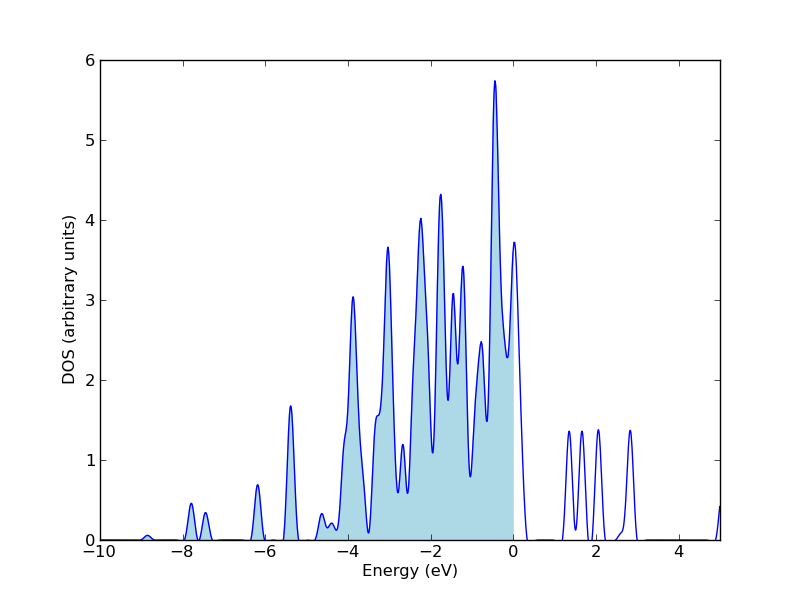
\includegraphics[width=4in]{./figures/Ni-total-DOS.png}
\caption{Total DOS of bulk Ni}
\end{figure}

\subsubsection{Looking at both spin up and spin down density of states}
\label{sec-3-2-2}
In systems with spin polarization, electrons can either be spin up or spin down. We can also look at the density of states of both the spin up and spin down electrons. This is done below.

\begin{minted}[frame=lines,fontsize=\scriptsize,linenos]{python}
from espresso import *
from ase.lattice import bulk
from ase.visualize import view
import matplotlib.pyplot as plt

atoms = bulk('Ni', 'fcc')

with Espresso('output/Ni', atoms=atoms, wf_collect=True,
              ecutwfc=40.0, ecutrho=500.0, kpts=(6, 6, 6),
              occupations='smearing', smearing='mp', degauss=0.01,
              nspin=2) as calc:
    fermi = calc.get_fermi_level()
    dos = EspressoDos(efermi=fermi) # Initialize the EspressoDos class which contains
                                    # all of the information needed to construct the
                                    # DOS

    E = dos.get_energies()          # Read an array of energies in which the DOS is constructed

    d_u = dos.get_total_dos(spin='+') # Read the spin up density of states at each energy in E
    d_d = dos.get_total_dos(spin='-') # Read the spin down density of states at each energy in E

    ind = (E < 5) & (E > -10)       # We're only concerned with the energies
                                    # near the fermi level

    occupied = (E < 0) & (E > -10)  # These are the occupied energy levels

plt.plot(E[ind], d_u[ind], c='b')        # Code for plotting the density of states
plt.plot(E[ind], -d_d[ind], c='b')       # Code for plotting the density of states
plt.fill_between(x=E[occupied], y1=d_u[occupied],
                 y2=np.zeros(E[occupied].shape), color='lightblue')                    
plt.fill_between(x=E[occupied], y1=-d_d[occupied],
                 y2=np.zeros(E[occupied].shape), color='lightblue')                    

plt.xlim(-10, 5)
plt.ylim(-3, 3)
plt.xlabel('Energy (eV)')
plt.ylabel('DOS (arbitrary units)')
plt.savefig('figures/Ni-total-spin-DOS.png')
plt.show()
\end{minted}

\begin{figure}[H]
\centering
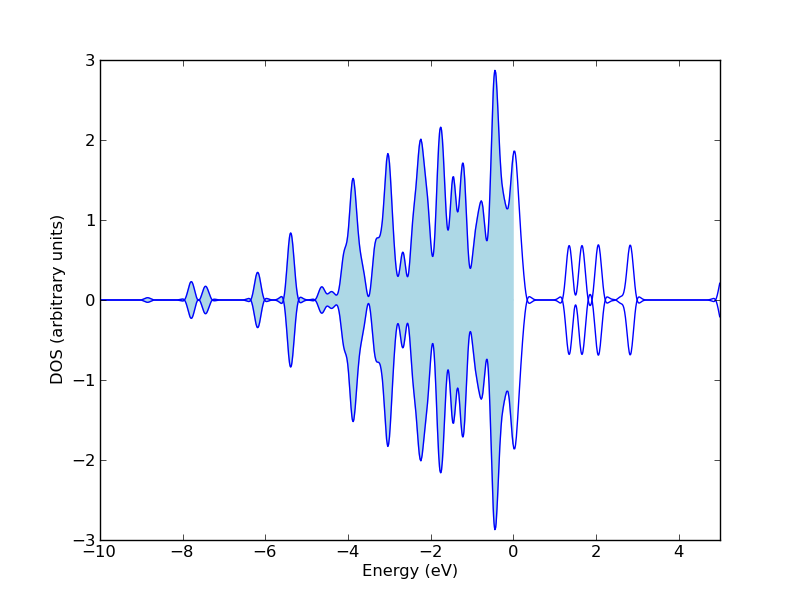
\includegraphics[width=4in]{./figures/Ni-total-spin-DOS.png}
\caption{Spin projected DOS of bulk Ni}
\end{figure}

\subsubsection{Looking at orbital projected density of states}
\label{sec-3-2-3}
One can also look at the orbital projected density of states of each atom. This is obtained via the \texttt{EspressoDos.get\_site\_dos} function. One needs to specify the index of the atom, the orbital desired, and whether you want the spin up, spin down, or both sets of electrons. Since the Ni fcc example only has one atom in the cell, its quite simple.

\begin{minted}[frame=lines,fontsize=\scriptsize,linenos]{python}
from espresso import *
from ase.lattice import bulk
import matplotlib.pyplot as plt

atoms = bulk('Ni', 'fcc', 3.52)

orbitals = ['3d', '4s']

colors = {'4s':['orange','y'],    # A dictionary of the orbitals and
          '3d':['b','lightblue']} # colors we want to graph them as.

with Espresso('output/Ni', atoms=atoms, wf_collect=True,
              ecutwfc=40.0, ecutrho=500.0,
              occupations='smearing', smearing='mp', degauss=0.01,
              nspin=2, kpts=(6, 6, 6), walltime='24:00:00', ppn=4) as calc:
    fermi = calc.get_fermi_level()
    dos = EspressoDos(efermi=fermi)
    energies = dos.get_energies()
    occupied = (energies < 0) & (energies > -10)
    for orb in orbitals:
        ind = (energies < 5) & (energies > -10)
        d = dos.get_site_dos(0, orb)
        
        plt.plot(energies[ind], d[ind], c=colors[orb][0], label=orb)
        plt.fill_between(x=energies[occupied], y1=d[occupied], 
                         y2=np.zeros(energies[occupied].shape),
                         color=colors[orb][1], label=orb)
plt.xlabel('Energy (eV)')
plt.ylabel('DOS (arbitrary units)')
plt.ylim(0, 6)
plt.savefig('figures/Ni-spin-proj-DOS.png')
plt.legend()
plt.show()
\end{minted}

\begin{figure}[H]
\centering
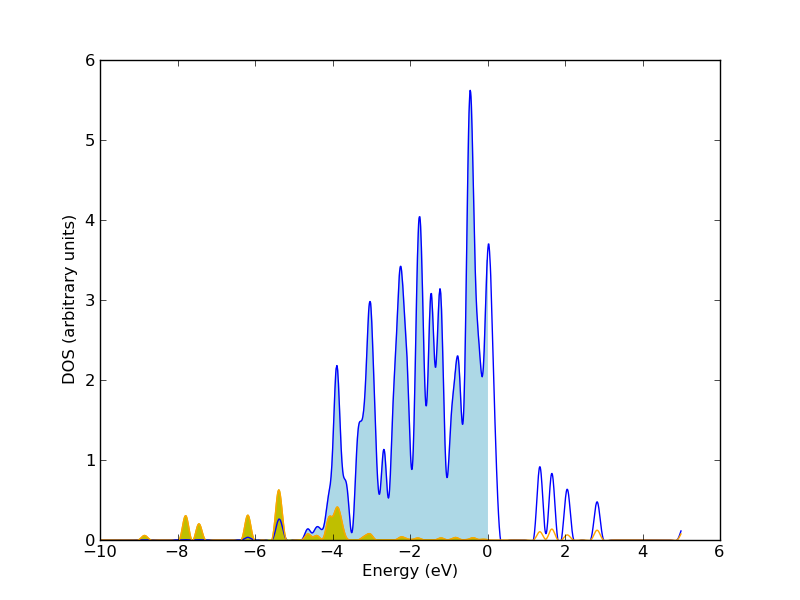
\includegraphics[width=4in]{./figures/Ni-spin-proj-DOS.png}
\caption{The spin projected DOS of bulk Ni}
\end{figure}

\subsubsection{An example with multiple atoms}
\label{sec-3-2-4}
We now look at an example with multiple atoms in the unit cell. We choose TiO2 in the rutile structure.

\begin{minted}[frame=lines,fontsize=\scriptsize,linenos]{python}
from espresso import *
from ase_addons.bulk import rutile
import matplotlib.pyplot as plt

atoms = rutile(('Ti', 'O'), a=4.65, c=2.97, u=0.31)

Ti_ind = [0, 1]
O_ind = [2, 3, 4, 5]

with Espresso('output/TiO2', atoms=atoms, wf_collect=True,
              ecutwfc=40.0, ecutrho=500.0, kpts=(6, 6, 6),
              occupations='smearing', smearing='mp', degauss=0.01,
              nspin=2, walltime='24:00:00', ppn=4) as calc:
    fermi=calc.get_fermi_level()
    dos = EspressoDos(efermi=fermi)
    E = dos.get_energies()
    occupied = (E < 0)
    d, p = np.zeros(len(E)), np.zeros(len(E))
    for i in Ti_ind:
        d += dos.get_site_dos(i, '3d')
    for i in O_ind:
        p += dos.get_site_dos(i, '2p')

plt.plot(E, p, c='r', label='O 2p')
plt.fill_between(x=E[occupied], y1=p[occupied],
                 y2=np.zeros(p[occupied].shape),
                 color='pink')
plt.plot(E, d, c='b', label='Ti 3d')
plt.fill_between(x=E[occupied], y1=d[occupied],
                 y2=np.zeros(d[occupied].shape),
                 color='lightblue')
plt.xlim(-10, 5)
plt.ylim(0, 12)
plt.xlabel('Energy (eV)')
plt.ylabel('DOS')
plt.legend(loc=2)
plt.savefig('figures/TiO2-DOS.png')
plt.show()
\end{minted}

\begin{figure}[H]
\centering
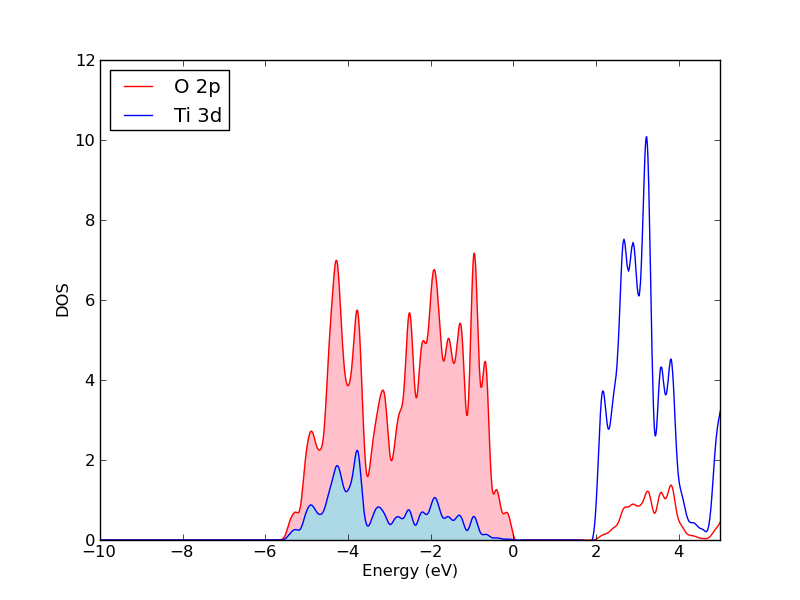
\includegraphics[width=4in]{./figures/TiO2-DOS.png}
\caption{Atom projected DOS of TiO2}
\end{figure}

\section{Parameter optimization}
\label{sec-4}
\section{Troubleshooting}
\label{sec-5}

\bibliography{../../Dropbox/bibliography/library}
% Emacs 24.3.2 (Org mode 8.2.6)
\end{document}